\documentclass[a4paper,11pt]{article}
\pdfoutput=1
\bibliographystyle{JHEP}
\usepackage[utf8]{inputenc}
\usepackage{jcappub}

\begin{document}
\title{\centering Colombian Network on High Energy Physics: Input on Theoretical HEP}

\author[a]{Mario A. Acero Ortega,}
\author[b]{Enrique Arrieta Díaz,}
\author[c]{Carlos Ávila,}
\author[d]{Juan P. Beltrán Almeida,}
\author[e]{Richard Benavides,}
\author[f]{Nicolás Bernal,}
\author[g]{Amalia Betancur,}
\author[h]{Andres Castillo,}
\author[d]{Raffaele Fazio,}
\author[c]{Andrés Flórez,}
\author[i]{David V. Forero,}
\author[j]{Diego Gallego,}
\author[k]{Yithsbey Giraldo,}
\author[h]{Luz Stella Gómez,}
\author[d]{Roberto Martínez,}
\author[l]{Jhovanny Andrés Mejía Guisado,}
\author[d]{Diego Milanés,}
\author[d]{John Morales,}
\author[f]{Deywis Moreno,}
\author[f]{Alexander Moreno Briceño,}
\author[f]{Gabriela Navarro,}
\author[d]{Fredy Ochoa,}
\author[d]{Carlos Quimbay,}
\author[l]{Diego Restrepo,}
\author[d]{Alexis Rodríguez,}
\author[k]{Eduardo Rojas,}
\author[l]{José David Ruiz Álvarez,}
\author[d]{Carlos Sandoval,}
\author[d]{Mauricio De Santis,}
\author[m]{César A. Valenzuela-Toledo,}
\author[l]{Nelson Vanegas,}
\author[j]{Carlos Yaguna,}
\author[l]{Óscar Zapata.}

\affiliation[a]{Universidad del Atlántico, Carrera 30 \# 8-49, Puerto Colombia}
\affiliation[b]{Universidad del Magdalena, Carrera 32 \# 22-08, Santa Marta}
\affiliation[c]{Universidad de los Andes, Cra. 1 No. 18A-10, Edificio Ip, Bogotá}
\affiliation[d]{Universidad Nacional de Colombia, Av. Cra 30 \# 45-03, Bogotá}
\affiliation[e]{ITM, Calle 73 \# 76A-354 , Vía el Volador, Medellín}
\affiliation[f]{Universidad Antonio Nariño, Cra 3 Este \# 47A-15, Bogotá}
\affiliation[g]{Universidad EIA, A.A. 7516, Envigado}
\affiliation[h]{Universidad Sergio Arboleda, Calle 74 \# 14-14, Bogotá}
\affiliation[i]{Universidad de Medellín, Carrera 87 \# 30, Medellín}
\affiliation[j]{UPTC, Avenida Central del Norte \# 39-115, Tunja}
\affiliation[k]{Universidad de Nariño, A.A. 1175, San Juan de Pasto}
\affiliation[l]{Universidad de Antioquia, Calle 70 \# 52-21, Medellín}
\affiliation[m]{Universidad del Valle, Ciudad Universitaria Meléndez, 760032, Santiago de Cali}


\emailAdd{nicolas.bernal@uan.edu.co}


\abstract{
This white paper presents the activities of the Colombian community concerning some theoretical aspects of high energy physics that are driving our research. In particular we want to highlight synergistic efforts done in the areas of dark matter, cosmology, flavor and hadron physics, and neutrino physics. This document summarizes the current status and interests of the different groups working on Theoretical High Energy Physics in Colombia, and their perspectives for the future.
}

\notoc
\maketitle

%%%%%%%%%%%%%%%%%%%%%%%%%%%%%%%%%%%%%%%%%%%%%%%%%%%%%%%%%%%%%%%%%
\section{Scientific Context}
The Colombian network on high energy physics (CONHEP) is a recent initiative created by the necessity of bringing together the Colombian community of high energy physics.
In fact, this community has steadily been growing in the last decade, with young scientists taking leading positions at local universities and more students joining this field of research. There are existing collaborations between different groups in the network, with researchers from different institutions working together. Research topics include flavour physics, beyond the standard model (SM) phenomenology, astroparticle physics, cosmology, dark matter (DM), and neutrino physics. In this context, we organize yearly since 2016 the Colombian meeting of high energy physics (COMHEP).

\subsection*{COMHEP}
The COMHEP is the annual Colombian meeting of high energy physics. We aim to bring together young and senior particle physicists from Colombia and abroad, to discuss recent progress in particle physics and related areas. The program of the meeting typically addresses a broad range of topics, such as: SM and beyond, neutrino physics, hadron and flavor physics, DM, cosmology, cosmic rays, and future experiments.
This year the fifth edition will take place:
\begin{itemize}
    \item \href{https://indico.cern.ch/e/comhep}{COMHEP 2016.} Nov. 28 - Dec. 2, 2016. Instituto Tecnológico Metropolitano.
    \item \href{https://indico.cern.ch/e/comhep2}{COMHEP 2017.} Dec. 4 - 7, 2017. Universidad Nacional de Colombia.
    \item \href{https://indico.cern.ch/e/comhep3}{COMHEP 2018.} Dec. 3 - 7, 2018. Universidad Santiago de Cali.
    \item \href{https://indico.cern.ch/e/comhep4}{COMHEP 2019.} Dec. 2 - 6, 2019. Universidad del Atlántico.
    \item \href{https://indico.cern.ch/e/comhep5}{COMHEP 2020.} Nov. 30 - Dec. 4, 2020. Online edition.
\end{itemize}

\noindent
In the following, we want to highlight four research areas in which the Colombian community is particularly active: dark matter, cosmology, flavour, and neutrino physics.\\

%%%%%%%%%%%%%%%%%%%%%%%%%%%%%%%%%%%%%%%%%%%%%%%%%%%%%%%%%%%%%%%%%\
\section{Identifying the New Physics of Dark Matter}
There is compelling evidence for the existence of DM, an unknown, non-baryonic matter component whose abundance in the Universe exceeds the amount of ordinary matter roughly by a factor of five. Still, the nongravitational nature of DM remains a mystery. The fact that the observed abundances of dark and visible matter are in the same ballpark may be considered as indicative that both forms of matter have a common origin and they were once in thermal equilibrium with each other. Despite the fact that DM has been searched for decades, the studies have yielded no overwhelming evidence for what DM actually is.\\

Here we want to highlight the main physics open questions that have been driving the research of our community, and what has been our role in the quest for unveiling them:%
\footnote{DM is one of the research subjects with the largest impact in Colombia, a conclusion endorsed by a recent publication in Nature~\cite{Bajak2018}.}

\begin{enumerate}
\item 
DM production in the early Universe
\begin{itemize}
\item 
WIMP mechanism\\
In the previous decades, this class of scenarios has received by far the biggest attention, both theoretically and experimentally. WIMPs (Weakly Interacting Massive Particles) typically carry electroweak scale mass and couple to the SM with a strength that is reminiscent to that of the weak interactions; the supersymmetric neutralino being the most studied~\cite{Masiero:2004vk, Profumo:2004at, Bernal:2007uv, Sierra:2009zq, Bernal:2009jc}.%
\footnote{See Ref.~\cite{Hirsch:2005ag} for a study with a thermally produced gravitino DM.}
The Colombian community has played a relevant role in both formulating and studying simplified DM scenarios~\cite{Yaguna:2008hd, Goudelis:2009zz, Honorez:2010re, LopezHonorez:2010tb, Alvares:2012qv, Esch:2013rta, ochoa, martinezg2, nisperuza, martinez, Arbelaez:2015ila, Horiuchi:2016tqw, Dutta:2017lny, Arbelaez:2017ptu}.\\
However, the nonobservation of WIMP DM puts this mechanism under a strong tension, both at theoretical and experimental levels. Among the different approaches to overcome the challenges on WIMP models, we recall those that depart from the standard cosmology scenario (see below), consider WIMPs to make up only a fraction of the total DM of the Universe~\cite{Betancur:2018xtj, Carvajal:2018ohk}, or multicomponent WIMP scenarios~\cite{Esch:2014jpa, Bernal:2018aon, Yaguna:2019cvp, Belanger:2020hyh}. 
\item
FIMP mechanism\\
The observed DM abundance may have been generated also out of equilibrium by the so-called freeze-in mechanism. In this scenario, the DM particle couples to the visible SM sector very weakly, so that it never entered chemical equilibrium. Instead, the DM particles were produced by decay or annihilation processes from the visible sector. Due to the small coupling strength, the DM particles produced via the freeze-in mechanism have been called Feebly Interacting Massive Particles (FIMPs).\\
The Colombian community has been particularly active in this front, pioneering studies on simplified models where the FIMP mechanism is realized~\cite{Yaguna:2011qn, Molinaro:2014lfa, Bernal:2018ins, Bernal:2018kcw} (see Ref.~\cite{Choi:2010jt,Restrepo:2011rj} for supersymmetric scenarios with gravitinos non-thermally produced).
Additionally, we have participated on understanding the impact of the details of the nonsudden reheating on the UV freeze-in~\cite{Bernal:2018qlk, Bernal:2020bfj, Bernal:2020gzm, Bernal:2020qyu}.
Finally, we have contributed to the only existing review on FIMP DM~\cite{Bernal:2017kxu}.
%
\item
SIMP mechanism\\
DM with strong self-interactions provides a compelling solution to several small-scale structure puzzles.
Under the assumption that the coupling between DM and the SM particles is suppressed, Strongly Interacting Massive Particles (SIMPs) allow for a successful dark freeze-out through $N$-to-$N'$ processes, where $N$ DM particles annihilate to $N'$ of them, with $N>N'\geq 2$.\\
Again, the Colombian community has been actively developing this alternative production mechanism, and looking for strategies allowing to test it, in particular with astrophysical and cosmological observables~\cite{Bernal:2015bla, Bernal:2015ova, Bernal:2015xba, Bernal:2017mqb, Bernal:2019uqr, Bernal:2020gzm}.
We want to highlight a review on the different production regimes for SIMPs and general self-interacting DM~\cite{Bernal:2015ova}.\\
Figure~\ref{fig:DM} shows a schematic representation of the regions where different DM production mechanisms (freeze-out, freeze-in, dark freeze-out, and reannihilation) dominate. The observed DM relic abundance is obtained on the dashed gray line, and the arrows show the gradient for DM abundance. The parameters $y$ and $\lambda$ are the DM coupling to the visible sector and the DM self-coupling, respectively.
\begin{figure}
	\centering
	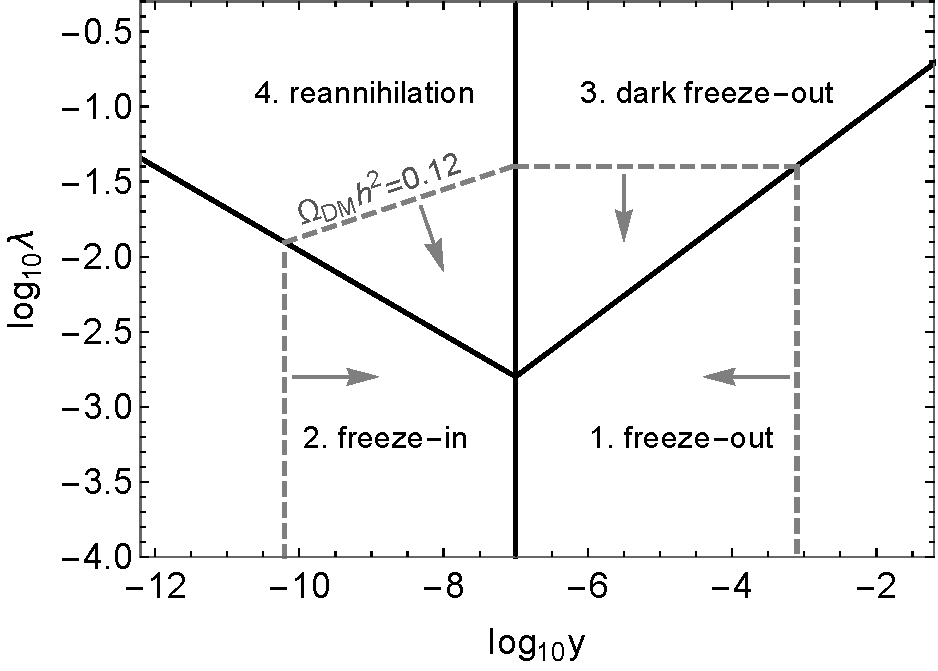
\includegraphics[scale=0.53]{plots/phases.pdf}
	\caption{A schematic representation of the regions where different DM production mechanisms dominate. The observed DM relic abundance is obtained on the dashed gray line, and the arrows show the gradient for DM abundance. The parameters $y$ and $\lambda$ are the DM coupling to the visible sector and the DM self-coupling, respectively.	Taken from Ref.~\cite{Bernal:2017kxu}.
	}
	\label{fig:DM}
\end{figure} 
%
\item
Axions\\
Axions and axion-like particles are also very popular DM candidates that could be related to the solution of the strong CP problem in QCD. A very light axion is stable and constitutes a natural DM candidate~\cite{yadir, Giraldo:2020hwl}.
%
\item
Nonstandard cosmologies\\
It is typically assumed that after inflation the evolution of the Universe is driven by the SM radiation energy density and that the SM entropy is conserved. However, that should not be the case. Alternatively, one can also consider nonstandard cosmological histories, for example, scenarios where the Universe was effectively matter-dominated at an early stage, due to a slow reheating period after inflation or to a massive metastable particle. There are no indispensable reasons to assume that the Universe was radiation-dominated prior to Big Bang nucleosynthesis. These scenarios drastically modify the prediction of cosmological abundances of particle species.\\
We have intensively studied this possibility in particle physics models looking for the enlarged parameter space compatible with the DM produced via different mechanisms in the early Universe~\cite{Bernal:2018kcw, Bernal:2018ins, Arias:2019uol, Bernal:2019mhf,Betancur:2018xtj}.
We want to highlight our contribution to a very recent review on the subject~\cite{Allahverdi:2020bys}.
\end{itemize}
%
\item
DM production at colliders
\begin{itemize}
\item
LHC phenomenology\\
New models, analysis techniques, and search strategies have been proposed to be conducted at the LHC. There is a significant number of articles published with strong involvement and leadership of Colombian scientists working on particle physics phenomenology at the LHC. For example, new ideas and models to explore the production of anapole DM~\cite{Florez:2019tqr}, heavy neutrinos as DM candidates~\cite{Andres:2017daw}, heavy mass neutral resonances~\cite{Andres:2016xbe, Abada:2018sfh}, gravitons~\cite{Florez:2018ojp}, two Higgs doublet models~\cite{Bernal:2009rk, LopezVal:2010vk}, DM in supersymmetric scenarios~\cite{Bernal:2007uv, Das:2017mqw, Avila:2018sja}, baryogenesis models~\cite{Bernal:2018nyv}, among others have been proposed. Additionally, new analysis techniques using vector boson fusion and initial state radiation jets~\cite{Florez:2016lwi}, have been proposed using simulated data. Several of these searches have later been conducted experimentally at the LHC.
%
\item 
DM searches with CMS\\
CMS (Compact Muon Solenoid) is a particle detector at the LHC. It has a broad physics program to search for physics beyond the SM, including DM. The effort of the experimental groups of the community involved concentrates on DM searches using supersymmetric models in compressed mass spectra scenarios with tau leptons. The searches are carried out using two different techniques,  vector boson fusion~\cite{Khachatryan:2015kxa, Khachatryan:2016mbu, Sirunyan:2019zfq} and jets from initial state radiation~\cite{Sirunyan:2019mlu}. In addition, the team has conducted searches for DM considering the production of heavy neutrinos with right-handed helicity in final states with tau leptons and jets~\cite{Sirunyan:2018vhk}. Finally, there has been also strong contribution in searches for heavy mass resonances decaying to tau leptons~\cite{Khachatryan:2016qkc}. It is important to mention that several papers have been published on these topics with strong involvement and leadership from the Colombian community.
%
\item
DM searches with DUNE\\
The Deep Underground Neutrino Experiment (DUNE) is an ambitious project currently under construction. The experiment will have a high-intensity proton beam, with either 60 or 120 GeV energies. Due to this high energy, it is possible to create a dark sector mediators or DM particles from meson decays. Such dark sector particles could then be detected at the near detector from their interactions with the liquid argon. Currently, Colombian institutions are developing models where DM particles interact via a dark photon. In this way, the dark photon could kinetically mix with the SM photon such as to generate interactions with the SM quarks or leptons that could be detected by the near detector's sensors. The goal is to impose constraints on the models that arise from different experiments (collider production, astrophysical experiments, etc), and then explore DUNE's sensitivity to the available parameter space.
\end{itemize}
%
\item
DM direct and indirect detection\\
Even if the Colombian community is not directly involved in any experimental collaboration aiming to directly or indirectly detect the DM particles, we make constantly use of their results~\cite{Bernal:2008zk, Bernal:2009tt, Bernal:2009jc, Sierra:2009zq, Choi:2010jt, Bernal:2010ip, Bernal:2011pz, Bernal:2012qh, Bernal:2012cd, martinez, Horiuchi:2016tqw}.
In particular, we have paid special attention to the role of galactic uncertainties in both direct and indirect detection~\cite{Bernal:2014mmt, Bernal:2016guq, Benito:2016kyp}.\\
As a community, we understand that the absence of a Colombian participation on the worldwide effort of detecting DM particles via direct and indirect detection experiments is a big issue that has to be solved in the near future.
%
\item
$N$-body simulations\\ 
According to astrophysics and cosmology, DM is a major constituent of the Universe that plays a fundamental role in the formation of structures and galaxies. This makes these astrophysical phenomena one of the best scenarios to study the DM nature. In that sense, $N$-body simulations of the structure formation and $N$-body simulations of the galactic dynamics become an important framework to study the properties and detectability of DM~\cite{Munoz-Cuartas2011, Maccio2013}.
The current $N$-body simulations of structure formation allow to study the spatial properties of DM, clustering and substructure abundance~\cite{Munoz-Cuartas2011b, Munoz-Cuartas2012}. All these subjects turn into important keys in the understanding of the properties of DM. In these simulations, standard ($\Lambda$CDM) and nonstandard (self-interacting, decaying DM, etc.) scenarios can be explored with the aim to contrast the predictions of many different physical scenarios against the observations.
Another subject where $N$-body simulations can shed light on the properties of DM is the study of dynamics of galaxies, and particularly merging galaxies~\cite{Norena_etal2019, Quiroga2020}. During these mergers, structures like streams, plumes, and rings of material emerge as a result of the gravitational interaction. The structure and dynamics of such structures depends closely on the properties of the DM and turns in a different scenario to study its properties~\cite{Quiroga2020}. A problem that can be tackled by making use of $N$-body simulations and that can be directly connected to what can be measured from observations~\cite{Bernal:2014mmt, Bernal:2016guq}.  
%
\item
Astrophysical and cosmological probes of DM\\
DM self-interactions could give a handle in solving long-standing problems in DM halos at small scales. Observations of the small-scale structure and cluster mergers may provide important insight into the nongravitational interactions inside the dark sector.
Additionally, isocurvature fluctuation modes are a generic feature of models where feebly coupled scalar fields exist in the dark sector. They arise from density fluctuations of dark sector scalar fields, in the case that the energy density stored in a scalar field at the end of inflation is deposited into DM. These modes are severely constrained by the CMB power spectrum.
Finally, the recent experimental success in observing gravitational waves has opened up a new avenue for observational cosmology, which will be further enhanced by, for example, the upcoming LISA mission. Gravitational waves produced in dark sector phase transitions could be observed with the LISA experiment, regardless of the weakness of nongravitational interactions between the dark and visible sectors~\cite{Almeida:2018oid, Bernal:2020bfj, Bernal:2020gzm, Bernal:2020qyu}.
%
\item
DM connections to other open problems beyond the SM
\begin{itemize}
\item 
Electroweak phase transitions\\
The presence of DM particles may induce significant changes on the scalar potential of the SM in such a way the electroweak symmetry breaking turns out to be a strong first-order phase transition. This feature would make viable electroweak baryogenesis as the solution to the matter antimatter asymmetry~\cite{Bernal:2009hd, Bernal:2017zvx}.
%
\item
Strong CP problem\\
The Peccei-Quinn solution to this problem brings along with the axion, which constitutes  a viable DM candidate. A possible link between the PQ symmetry as the stabilizing symmetry of the WIMP DM particles has been explored in Refs.~\cite{Ma:2017zyb, Carvajal:2018ohk}.  
%
\item
Neutrino masses\\
Heavy new particles usually used to explain the smallness of neutrino masses can be easily accommodated in the dark sector where the lightest particle can be identified as the DM particle.\\
The Colombian community has been very prolific in studying this kind of scenarios~\cite{Bernal:2017xat}, in particular the so-called ``scotogenic'' model. One of the first systematic analysis addressing the DM problem in radiative neutrino mass models was presented in Ref.~\cite{Restrepo:2013aga}, drawing the attention of the community for this kind of analysis. In a subsequent analysis~\cite{Calle:2018ovc} it was shown that all the one-loop realizations of the dimension-5 operator to effectively generate Dirac neutrino masses can be implemented by using a single local $U(1)$ symmetry, with some of them being a viable DM candidate.
Additionally, in Ref.~\cite{Calle:2019mxn} a minimal implementation of the radiative type-I seesaw with light Dirac neutrinos and heavy Majorana fermions was presented. On the other hand, the phenomenology of several scotogenic models has been carried out~\cite{Sierra:2008wj, Molinaro:2014lfa, Restrepo:2015ura, Ibarra:2016dlb, vonderPahlen:2016cbw, Betancur:2017dhy, Reig:2018mdk, Reig:2018ztc, Bernal:2018aon, Restrepo:2019soi, Restrepo:2019ilz}.
%
\item
Inflation\\
Potential connections between DM and the inflationary dynamics have recently been subject of study of our community.
In particular, DM genesis could have taken place during the reheating, before the onset of the radiation domination era~\cite{Bernal:2018hjm, Bernal:2018qlk, Bernal:2020bfj, Bernal:2020qyu}.
Alternatively, the field responsible for the early expansion period of the Universe (the inflaton) may serve as a DM candidate~\cite{Almeida:2018oid}.
%
\item
Baryon asymmetry of the Universe\\
The fact that the ratio of the abundances of dark and baryonic matter is a number not far from one, would suggest a common mechanism for the origin of the two species.
The Colombian community has been working on scenarios where the DM genesis is closely related to the baryon asymmetry on the Universe, in particular in the WIMPy baryogenesis model~\cite{Bernal:2012gv, Bernal:2013bga, Bernal:2016gfn, Bernal:2017zvx}.
\end{itemize}
\end{enumerate}
%
\subsection*{MOCa (Materia Oscura en Colombia)}
The Colombian workshop on DM (MOCa) is an initiative that arises as a response  to the need to strengthen the Colombian community working on several aspects related to the DM. It is important to mention that in the country we are reaching a critical mass, and we are already working on different subjects like particle physics, cosmology, and astrophysics, but also in the theoretical, experimental and phenomenological fronts. In that sense, DM can be used as an opportunity to make contact between our different expertise, even if for all of us DM is not the main research area.\\
This year, the workshop is having its fourth edition:
\begin{itemize}
\item \href{https://forero.github.io/MOCA/}{MOCa 2017.}
Jun. 17 - 29, 2017. %19 participants and 12 talks.
%
\item
\href{https://indico.cern.ch/e/moca2018}{MOCa 2018.}
Jul. 30 - Aug. 1, 2018. %73 participants and 18 talks.
%
\item
\href{https://indico.cern.ch/e/moca2019}{MOCa 2019.}
Sep. 30 - Oct. 2, 2019. %56 participants and 17 talks. This edition counted with two international invited speakers: Prof. Chee Sheng Fong (UFABC, Brazil) and Prof. James Unwin (Illinois U., USA).
%
\item
\href{https://indico.cern.ch/e/moca2020}{MOCa 2020.}
Oct. 7 - 8, 2020. Online edition.
\end{itemize}
%
The workshop so far has been held by Universidad de los Andes and has received financial support by Universidad de los Andes, Universidad Antonio Nariño, ICTP, and MinCiencias. These funds are essential especially for supporting students with travel and local expenses.
%This meeting will continue in the forthcoming years and, more importantly, will be enlarged with a day devoted to introductory lectures for early stage students interested in the field.
This year, the workshop will be preceded by the \href{https://fisindico.uniandes.edu.co/event/18/}{6$^\text{th}$ Uniandes particle physics school}. Students are warmly invited to attend.
%Organizers: Carlos Ávila (Universidad de los Andes), Juan Pablo Beltrán (Universidad Nacional de Colombia), Nicolás Bernal (Universidad Antonio Nariño), Andrés Flórez (Universidad de los Andes), Jaime Forero (Universidad de los Andes) and César Valenzuela (Universidad del Valle).


%%%%%%%%%%%%%%%%%%%%%%%%%%%%%%%%%%%%%%%%%%%%%%%%%%%%%%%%%%%%%%%%%\
\section{Understanding the Cosmic Acceleration}
Cosmology is living an exciting age due to the vast amount of data coming from present and planned missions devoted to measure the distribution of primordial cosmological (temperature) perturbations in  the cosmic microwave background (CMB), and the large scale structures (LSS) in the Universe. This data are making possible for the first time in history to test, compare, constraint and eventually rule out several models proposed as candidates to explain the mechanisms driving the beginning and evolution at large scales of the Universe. 

Following the excitement about the latest advances in the field, the Colombian community has been engaged in several research projects in theoretical cosmology over the last years. Several local and international collaborations have been created and maintained over the years in a wide and diverse spectrum of research interests ranging from inflationary physics to details of the LSS formation process. In the following, we highlight the main physics open questions that have been driving the research of our community:
\begin{enumerate}
\item 
Inflation\\
Inflation is the current paradigm in cosmology which describes the main features of the early Universe and solves the pressing problems related to fine tuning and causality of the initial conditions of the Big Bang model. The simplest and most successful version of this mechanism requires a single scalar field to drive an exponentially accelerated expansion able to smooth the initial conditions of the Universe and, because of its quantum fluctuations, to generate irregularities in the energy density after horizon exit. Afterwards, via gravitational clustering, it generates the large-scale structure that is seen today. The inflationary mechanism is simple and is able to explain most of the features of the CMB; however, when studying the different implementations of the inflationary idea, we recognize that there is generally a lack of connection of this physics with the low-energy particle physics accessible to current experiments. This difficulty is mainly due to the vastly different energy scales between inflation and particle physics processes.
The Colombian community has been actively working on possible connections between the inflationary dynamics and the particle physics~\cite{Bernal:2018hjm, Almeida:2018oid, Bernal:2020bfj, Bernal:2020qyu, Almeida:2020kaq}.\\
The precise measurements of CMB anisotropies impose strong constraints on the primordial power spectrum at scales 0.008~Mpc$^{-1}\lesssim k \lesssim 0.1$~Mpc$^{-1}$, providing exquisite information on the first 7 $e$-folds of inflation. This range of knowledge is extended to about 20 $e$-folds by measurements of Lyman-$\alpha$ forest and $\mu$ spectral distortions, which are sensitive to the integrated scalar power spectrum in the range 50~Mpc$^{-1}\lesssim k\lesssim 10^4$~Mpc$^{-1}$. The left panel of
Fig.~\ref{fig:cosmo} shows an example of power spectra fulfilling the observational constraints~\cite{Almeida:2020kaq}.
\begin{figure}
	\centering
	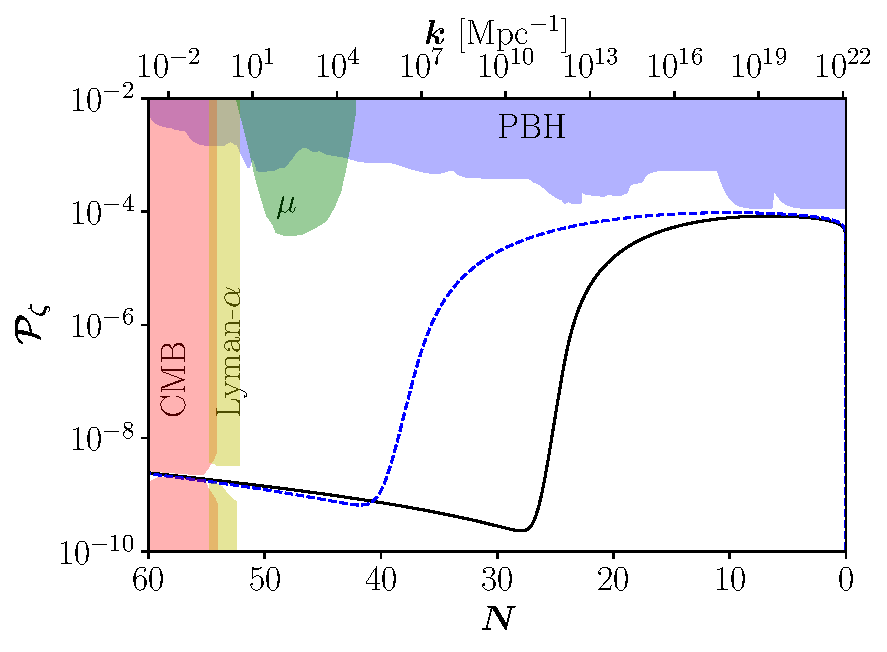
\includegraphics[scale=0.55]{plots/spectrum.pdf}
	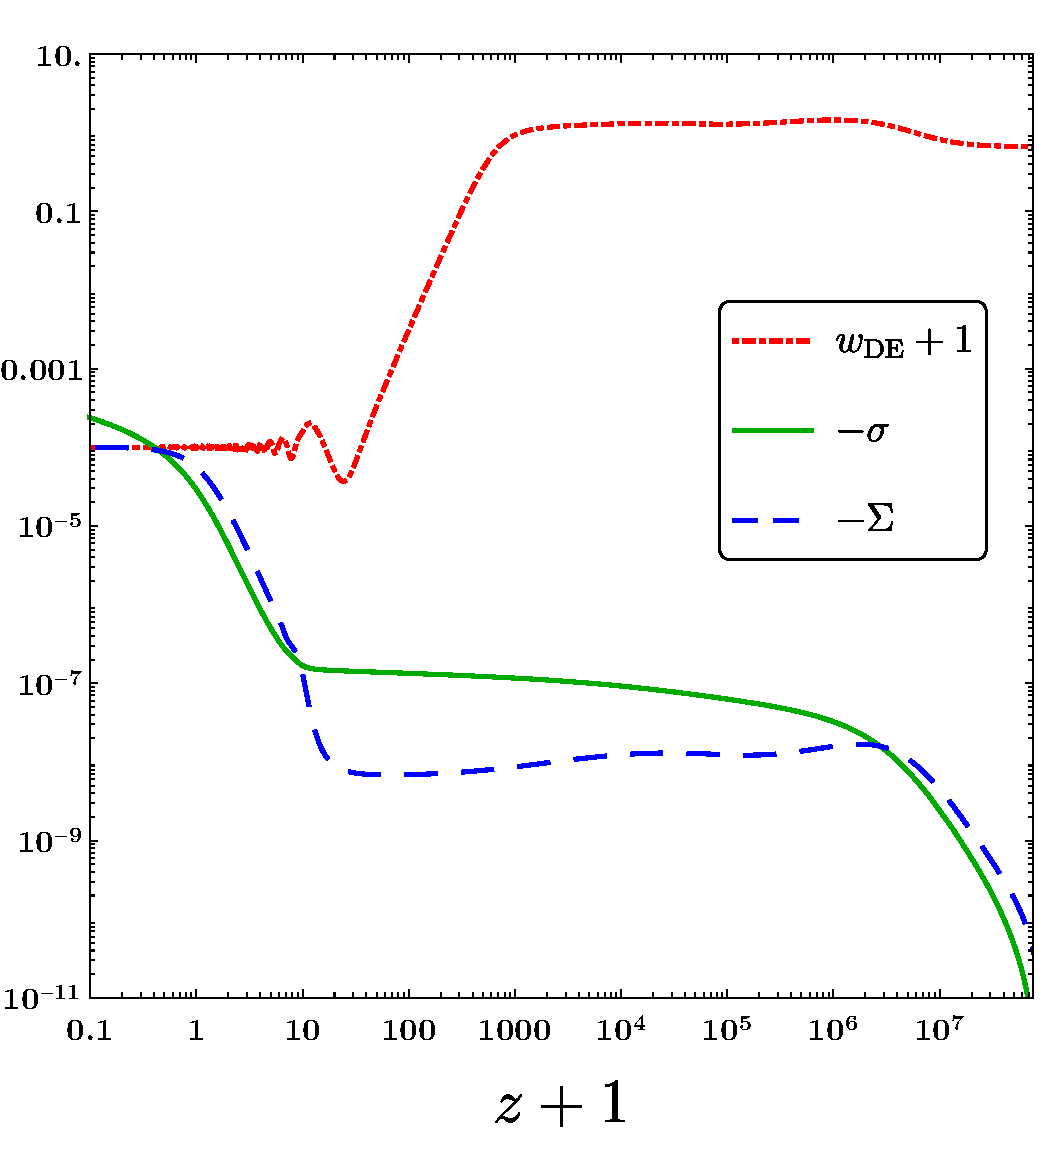
\includegraphics[scale=0.32]{plots/ltsigma.pdf}
	\caption{Left panel: Scalar spectra.  The colored regions are excluded by CMB anisotropies (red), Lyman-$\alpha$ forest (yellow), $\mu$ distortions (green) and PBH bounds (blue). Taken from Ref.~\cite{Almeida:2020kaq}.
	Right panel: Evolution of non-vanishing anisotropic shear in a DE model in the presence of a $2$-form field coupled to a scalar field. Taken from Ref.~\cite{Almeida:2019iqp}. }
	\label{fig:cosmo}
\end{figure} 
%
%\item
%Reheating\\
%At the end of inflation, the Universe has grown by a factor of around 60 $e$-folds and is essentially empty. During reheating, the energy density of the inflaton is converted into SM radiation. Several constraints apply in order to have a successful heating period. In particular, it is desirable that not a great amount of dark radiation is generated during reheating and instead the energy stored in the inflaton is effectively populating via the observable sector~\cite{Bernal:2020bfj, Bernal:2020qyu}. 
%
\item
Modified gravity theories\\
Modified gravity theories generalize Einstein's general relativity.
%In modified gravity theories, it is desirable to reduce the number of free parameters, or better, to have a model-independent way to test large families of theories.
In this context, the Colombian community has focused on the study of different models, and in particular on Horndeski-like theories. In this context, there is a model-independent observable called the anisotropic stress $\eta$ (or also called gravitational slip). By combining galaxy clustering and weak lensing probes (the core tools of an Euclid-like survey), a forecast analysis can be carried out to constrain the precision within which the anisotropic stress could be measured~\cite{Amendola:2013qna}. Additional applications of modified gravity models of current interest for the local groups are astrophysical solutions like black holes and compact objects, inflationary solutions, among others. 
%
\item
Non-Gaussianity and symmetry breaking patterns in the CMB\\
The interest in these subjects is justified by the fact that non-Gaussianity (NG) and statistical anisotropy signatures in the probability distribution of the CMB temperature anisotropies are sensitive to the specific details of the mechanisms ruling the dynamics of the early Universe. Thus, their precise evaluation could provide relevant criteria to discriminate among the many models proposed to explain the origin of the observed LSS distribution. Moreover, the detection of a significant signal of NG and statistical anisotropy would rule out the simplest models of inflation based on a single ``slowly rolling'' scalar field driving the inflationary mechanism. A possible way to generate significant levels of statistical anisotropy and NG particularly well studied by the Colombian community, is by introducing vector fields, antisymmetric tensor fields ($p$-forms), or general gauge fields during the inflationary epoch as a source of the primordial curvature perturbation~\cite{ValenzuelaToledo:2009af, ValenzuelaToledo:2009nq, ValenzuelaToledo:2011fj, BeltranAlmeida:2011db, Rodriguez:2013cj, Almeida:2014ava, Fleury:2014qfa, Almeida:2017lrq, Almeida:2019xzt, Almeida:2019hhx}.
%
\item
Primordial and astrophysical gravitational waves\\
The recent observations of gravitational waves by LIGO and Virgo paved the way to observe the Universe with new methods not based on electromagnetic radiation. The existence of a PGW background is one of the most crucial predictions of the inflationary scenario of the early Universe. Future gravitational wave observatories like the Einstein Telescope, LISA or BBO, and pulsar timing arrays could start probing the relevant parameter space favoured by a number of inflationary models.
Primordial gravitational waves can be considered as a smoking gun of inflation. Several models of inflation predict specific patterns and amplitudes for the gravitational waves produced during the inflationary epoch. Currently, some local groups have interest in inflationary models in the presence of additional degrees of freedom aside from the inflaton scalar field. Those models include typically couplings with gauge fields and non-minimal couplings with gravity. The particular features of the gravitational waves depend on the particular kind of coupling and can be constrained with CMB data~\cite{Almeida:2018pir, Bernal:2019lpc, Almeida:2020kaq}.  
%
%\item
%Large Scale Structures Formation\\
%LSS of the Universe refers to the distribution of matter in the largest observable scales that is bound together by the gravitational force. Structure formation is the process where a tiny spatial perturbation in the matter distribution becomes more inhomogeneous with the passage of time, due to the gravitational instability of matter, until galaxies, clusters of galaxies and superclusters are formed. The widely accepted mechanism to seed the Universe with initially tiny matter inhomogeneities is cosmological inflation. The current and future experiments will allow us to build a three-dimensional map of the structures that make up our Universe. With the data from these missions, we expect to have a precise temporal evolution of the growth of the structures at cosmological scales, which will allow, for example, to an accurate description of the dark energy. 
%
\item
Dark Energy\\
In the late 90s, two independent groups discovered that the Universe is actually engaging into a period of accelerated expansion. Since then, a number of theoretical avenues have been investigated to explain it. Although the simplest explanation is in favour of a cosmological constant, its required value is very small when compared with theoretical expectations that other alternatives have been put forward to explain the observed cosmic acceleration without having to resort to unnaturally small parameters. The two most popular alternatives to a cosmological constant are the dark energy, a hypothesized new form of matter making up about 68\% of the Universe's energy, and the modification of the theory of gravity allowed due to the poor experimental constraints of the general relativity theory on large scales. Currently, these alternatives remain plausible explanations of the cosmic acceleration and, however, they entail radically different implications for the physical theories describing nature. Owing to this, the discovery of the agent causing the late-time cosmic acceleration (either cosmological constant, dark energy or modified gravity) has become one of the most pressing questions in theoretical cosmology. Several dynamical dark energy models have been studied by local research groups aiming to propose alternative candidates beyond a single scalar dark energy field model~\cite{Rodriguez:2017wkg, Alvarez:2019ues, Almeida:2020lsn, Gomez:2020sfz, Orjuela-Quintana:2020klr, Guarnizo:2020pkj}, or estimate the impact of additional degrees of freedom such as gauge fields and $p$-forms in the dynamics of dark energy~\cite{Almeida:2018fwe, Almeida:2019iqp}. As an example of the later, the right panel of Fig.~\ref{fig:cosmo}  shows the evolution of anisotropic shear in a 2-form model of dark energy consistent with current observational limits for cosmological parameters.   
%
%\item
%UV completions\\
%From the perspective of a consistent quantum description, one has to rely on models resulting, for example, from string compactifications. These models, despite being in principle consistent, come with many extra ingredients, for example, several scalar fields and definite couplings with the matter sector. This not only allows to rule out plenty of models but also the construction of models not proposed yet.  Although the problem has many points to tackle in general these are encoded in what is called modular cosmology,  where the moduli fields can play the role of the inflaton, and in general might produce unwanted NG, but also can help to explain a tiny value for the cosmological constant and, since all these scenarios are in a supergravity playground, to break supersymmetry at some stage.
\end{enumerate}

\subsection*{CoCo (Cosmología en Colombia)}
The Colombian workshop on cosmology (CoCo) is an initiative that arises as a response  to the need to strengthen the Colombian community working on several cosmological aspects. It is important to mention that in the country we are reaching a critical mass, and we are already working on different subjects like inflation, black holes, dark energy, modified gravity, gravitational waves, LSS, $N$-body simulations, and the connection with particle physics. In that sense, cosmology can be used as an opportunity to make contact between our different expertise.\\
This year the workshop will have its second edition:
\begin{itemize}
\item 
\href{https://indico.cern.ch/e/coco2019}{CoCo 2019.}
May 30 - 31, 2019. %67 participants and 33 talks. This first edition counted with an international invited speaker: Prof. Sergio Palomares-Ruiz (IFIC, Spain).
%
\item
\href{https://indico.cern.ch/e/coco2020}{CoCo 2o2o.}
Sep. 23 - 25, 2020. Online edition. 
\end{itemize}

The workshop was held and funded by Universidad Antonio Nariño. 
This meeting will continue in the forthcoming years and, more importantly, will be enlarged with a day devoted to introductory lectures for early stage students interested in the field.
%Organizers: Juan Pablo Beltrán (Universidad Nacional de Colombia) and Nicolás Bernal (Universidad Antonio Nariño).




%%%%%%%%%%%%%%%%%%%%%%%%%%%%%%%%%%%%%%%%%%%%%%%%%%%%%%%%%%%%%%%%%\
\section{Flavor Physics as a Tool for Discovery}
The SM represents the best theory to describe electric and magnetic forces in a unified picture with the weak and the strong forces. However, there are many questions that so far do not have a definitive answer.  For example, in the quark sector, there are 10 unknown parameters, 6 masses, 3 mixing angles, and one phase; an equal number of parameters (or even larger for Majorana neutrinos) is needed in the lepton sector. The exact mechanism originating these scales is unknown; however; over the last decades, several models that address these questions have been proposed. In general, the mechanism that explains these mass scales is part of the so-called flavor problem.
%
\begin{enumerate}
\item 
Beyond the SM and flavor physics
\begin{itemize}
\item 
Electroweak extensions of the SM\\
Some of these questions can be answered by introducing an additional electroweak sector. In particular, flavored symmetries result quite useful to address the replication problem, the mass hierarchy, and even charge quantization. The idea heavily relies on the cancellation of the chiral anomalies, which represent quantum constraints on the gauge charges of the chiral models~\cite{unalfisicaunaldep, unalfisicaunaldepa, unalfisicaunaldepar, unalfisicaunaldepart, unalfisicaunaldeparta, unalfisicaunaldepartam, unalfisicaunaldepartame}.  It is important to highlight that many research groups in Colombia have worked on 331 models and on models with a nonuniversal $Z'$ which usually are suitable to address flavor problems~\cite{unalf, Diaz:2004fs, unalfis, unalfisi, unalfisic, unalfisica, unalfisicau, unalfisicaun, unalfisicauna, unalfisicaunal, unalfisicaunald, unalfisicaunalde, Benavides:2018rgh, Benavides:2018fzm, Rodriguez:2016cgr,Salazar:2015gxa}. 
It is important to highlight the lasting contribution to  the classification of the electroweak extensions of the standard model by the Colombian  groups~\cite{Ponce:2002sg, Diaz:2004fs, Rojas:2015tqa, Benavides:2016utf, Benavides:2018fzm}.
%
\item
Discrete and global symmetries\\
Discrete and global symmetries result quite useful to explain the SM mass scales and CP-violating phases.  In many cases, it is possible to obtain these symmetries as residual symmetries of gauge group interactions mediated by heavy gauge bosons. In this way, the low energy accidental symmetries could shed light on the underlying physics principles and symmetries at very high energies.  The same is true in the phenomenological analysis of the texture-zeros in the quark and lepton mass matrices, which can be considered in many cases as alternatives to impose discrete symmetries~\cite{Giraldo:2011ya, unalfisicaunaldis, unalfisicaunaldisc, unalfisicaunaldiscr, unalfisicaunaldiscre, Benavides:2020pjx}. 
\end{itemize}
%
\item
Flavor and hadron physics
\begin{itemize}
\item 
Flavored bound states\\
Since the fundamental degrees of freedom of the strong interaction, quarks and gluons, cannot propagate freely through the  vacuum, the only states with well-defined properties at low energies are singlet-color states.  The properties of these states are determined by the content of quarks and by the representation of the flavor group to which they belong. Owing to the  fact that many of these states are not flavor singlets, all the possible flavor combinations  generate a zoo of particles whose spectrum can be explained as bound states of  the lighter quarks.
On these topics, the Colombian community has contributed to the calculation of the meson spectrum, its decay constants, and its electromagnetic properties in the Bethe-Salpeter and Schwinger-Dyson formalism~\cite{Rojas:2013tza, Rojas:2014aka, Rojas:2014tya, Segovia:2015hra, El-Bennich:2016bno, Mojica:2017tvh, Molina:2020zao}.
Many of these states have a net weak charge. That is important for  hydrogen-like atoms since that, in that case, it is possible to make precise theoretical predictions. The strongest constraints on the $Z\text{-}Z'$ mixing angle come from the precise measurements of the cesium weak charge~\cite{Erler:2009jh}.
\item
Flavor changing neutral currents (FCNC)\\
In the SM,  the GIM mechanism avoids FCNC at the tree level; however, it is possible to have FCNC at loops order. The precise measurements of these processes represent strong constraints on the electroweak extensions of the SM.
One of the consequences of the family-dependent charges is the  FCNC at the tree level, 
the strongest constraints on these phenomena come from the $K^0$-$\bar K^0$ mixing, leptonic and semileptonic meson decays and coherent $\mu$-$e$ conversion in a muonic atom~\cite{Benavides:2018rgh, Langacker:2000ju}, which impose tough restrictions on the new-physics couplings to the left-handed quark doublets of the first and second generations~\cite{LopezCastro:1998fr, Larios:2004mx, CarcamoHernandez:2005ka, Benavides:2018rgh}.
Flavored axions are also a source of FCNC~\cite{DiLuzio:2020wdo}, these models are useful to understand, simultaneously,  the strong CP problem and the origin of the mass hierarchies in the SM~\cite{Garnica:2019hvn}. The most general expressions for the tree-level FCNC couplings between an axion-like particle and the SM fermions have been reported in Ref.~\cite{Giraldo:2020hwl}.
Clear signals of new physics are also expected from lepton-number-violating decays of heavy flavors~\cite{Delepine:2012nea, Castro:2012gi, Castro:2012ma, Quintero:2012jy, Quintero:2016iwi, Mejia-Guisao:2017nzx}.
%
\item
Lepton universality violation in  the $B$ meson decays\\ 
The $B$ meson decays have constituted a good scenario for studying, on both theoretical and experimental levels, the SM as well as for exploring new physics (NP) effects at low-energy scales. Particularly, semileptonic and leptonic $B$ meson decays offer an excellent place to test lepton universality (LU), so far one of the cornerstones of the SM. Any mismatch between the theoretical and experimental predictions may be an indication of LU violation, and therefore a hint of NP beyond the SM~\cite{Bernal:2011pj, Greljo:2018tzh, Benavides:2018rgh, Gomez:2019xfw, Cardozo:2020uol}.
%
%\item
%Measurements on spectroscopy and heavy flavor with CMS\\
%CMS has a broad physics program, including Measurements on spectroscopy and heavy flavor, and search for physics beyond the SM. The experimental groups of the community are involved in leptonic $B$ meson decay, which offers excellent opportunities to perform precision tests of the SM of particle physics because of minimal hadronic uncertainties in the theoretical predictions. On the other hand, although QCD is well established as the theory of the strong interaction, a complete understanding of the (nonperturbative) processes that lead to the binding of quarks and gluons into hadrons is still lacking. The $B_c$ family consists of charged mesons composed of a beauty quark and a charm antiquark (or vice versa), and the bottomonium family, composed of beauty quark-antiquark bound states, play a special role in understanding how the strong force binds quarks into hadrons. It is important to say that our groups are strongly involved in this research field and several of the results released by the CMS collaboration on these issues were led by our researchers.  
\end{itemize}
\end{enumerate}

\section{Identifying New Physics at Neutrino Experiments}
%
Neutrino oscillations, together with the existence of DM, provide striking evidence for physics beyond the SM. Neutrino oscillations imply nonzero neutrino masses, which in turn implies that the SM must be extended. Many realizations of the so-called dimension five operator can be found in the literature. A popular option to generate neutrino masses is known as the seesaw mechanism, although other possibilities can be considered as well, for instance, radiative models. Thus, the question of the origin of the neutrino mass is still open.

From the theoretical point of view, the nature of the neutrino (whether it is a Dirac or a Majorana particle) is another big open question and many experimental efforts are focused on the observation of the neutrinoless double beta decay process. An observation of this process implies that neutrinos are Majorana particles. Last, but not least, the existence of extra neutrinos that do not couple to the SM gauge bosons, which can span different energy scales, has also attracted the attention of the community. In particular, an sterile neutrino at the eV scale, motivated by several anomalies (e.g. short baseline~\cite{Aguilar:2001ty, Aguilar-Arevalo:2013pmq}, reactor antineutrino~\cite{Mueller:2011nm} and gallium~\cite{Acero:2007su, Giunti:2010zu} experiments), has become one of the priorities in the present and future neutrino program. Thus, even though in the last years much progress has been made to unveil several neutrino properties, some questions are waiting to be answered with the results of current and future facilities.

In what follows, we concentrate on {\it neutrino oscillations,} first, highlighting what it is known and the efforts to measure the unknowns, and second, mentioning examples where it has become a tool to explore beyond the SM physics. In each of the next topics, the main contributions from the Colombian scientists are highlighted.

\begin{enumerate}
    \item The three active neutrino oscillation framework
    \begin{itemize}
        \item The observation of neutrino oscillations from several sources has allowed the determination of the two mass-squared differences (historically named as solar and atmospheric), and the three mixing angles. These parameters are determined by the global combination of the existing data measured at different neutrino oscillation experiments. Currently, these parameters are determined within the 3\%-6\% of precision~\cite{deSalas:2020pgw}.
        \item Within this framework there is an important parameter yet to be determined, the Dirac CP phase, which encodes the possibility that the CP symmetry is violated in the leptonic sector. In addition, with three active neutrinos, there are two possible neutrino mass orderings depending upon whether the third mass eigenstate is the largest (smallest) of the three mass eigenstates, corresponding to normal (inverted) neutrino mass ordering. Although current experiments like T2K, NOvA (at which the Colombian community contributes~\cite{NOvA:2018gge,Acero:2018kyq,Acero:2019ksn}), atmospheric  (combined with reactor experiments), provide some preference for certain CP-violating values (cf. Fig.~\ref{fig:nova}), there is not a concluding measurement. In addition, there is no conclusive information on the neutrino mass ordering. For this reason, future neutrino facilities like DUNE and Hyper-K are being planned to measure the current unknowns and to improve the precision of the parameters already measured. 
        \begin{figure}
	    \centering
	    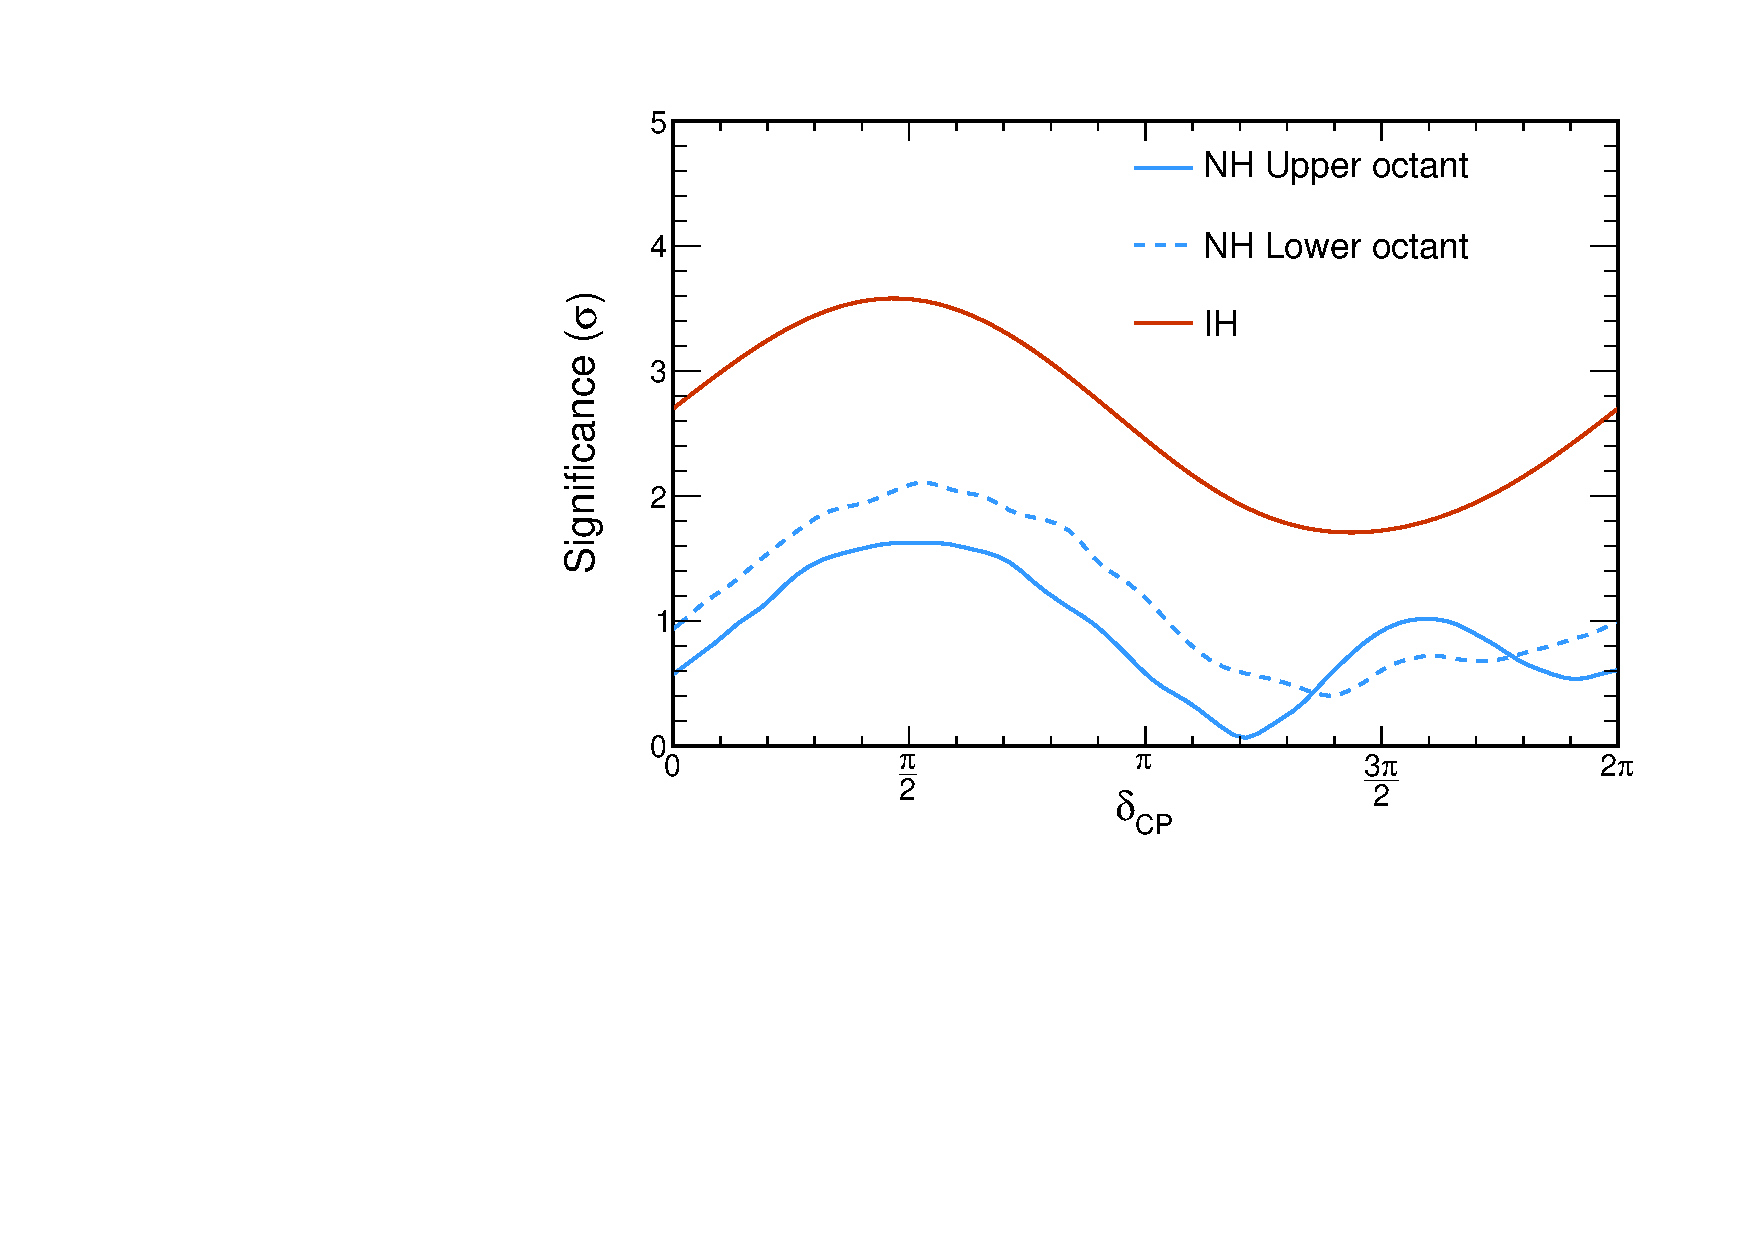
\includegraphics[scale=0.55]{plots/slice_delta_3curves.pdf}
	    \caption{NOvA results on the significance at which each value of $\delta_\text{CP}$ is disfavored in the normal (blue, lower) or inverted (red, upper) mass hierarchy. The normal mass hierarchy is divided into upper (solid) and lower (dashed) $\theta_{23}$ octants corresponding to the near degeneracy in $\sin^2\theta_{23}$.  Taken from Ref.~\cite{NOvA:2018gge}.}
    	\label{fig:nova}
        \end{figure} 
        Additionally, Colombian researchers are actively participating, contributing to relevant aspects of the detector system and the oscillation neutrino program~\cite{Abi:2020wmh, Abi:2020evt, Abi:2020qib}.
%        \item Some neutrino properties can not be known only through neutrino oscillations, such as the two Majorana phases (in case neutrinos are Majorana particles) and the absolute neutrino masses. Thus, complementary information coming from the observation of other processes like single beta decay, neutrinoless double beta decay, and cosmology become relevant. This opens the door to explore the synergies with other particle physics phenomena and other areas like astrophysics and cosmology.
    \end{itemize}
    \item Beyond the three active neutrino oscillation framework
    \begin{itemize}
        \item Neutrinos might have interactions that are not part of the SM. For instance, to generate neutrino masses, new fields have to be added to the SM fields, and they might be at scales above (or close to) the electroweak breaking scale, and therefore they can modify the SM physics at low energies. For phenomenological studies, there is a common framework in the form of effective dimension six and eight operators that increase the couplings to neutrinos in comparison to the SM ones. This is the so-called Nonstandard Neutrino Interactions (NSI). NSI can modify any of the three stages in a neutrino oscillation experiment, i.e., production, propagation, and detection. There are plenty of phenomenological works constraining these new couplings. Of particular interest, since the NSI couplings are complex in general, they might provide new sources of CP violation. It is then interesting to establish the robustness of the six neutrino oscillation parameters under the NSI and whether the undetermined Dirac CP violation can be obtained from a nonstandard source~\cite{Forero:2016cmb}.
    \begin{figure}
	\centering
	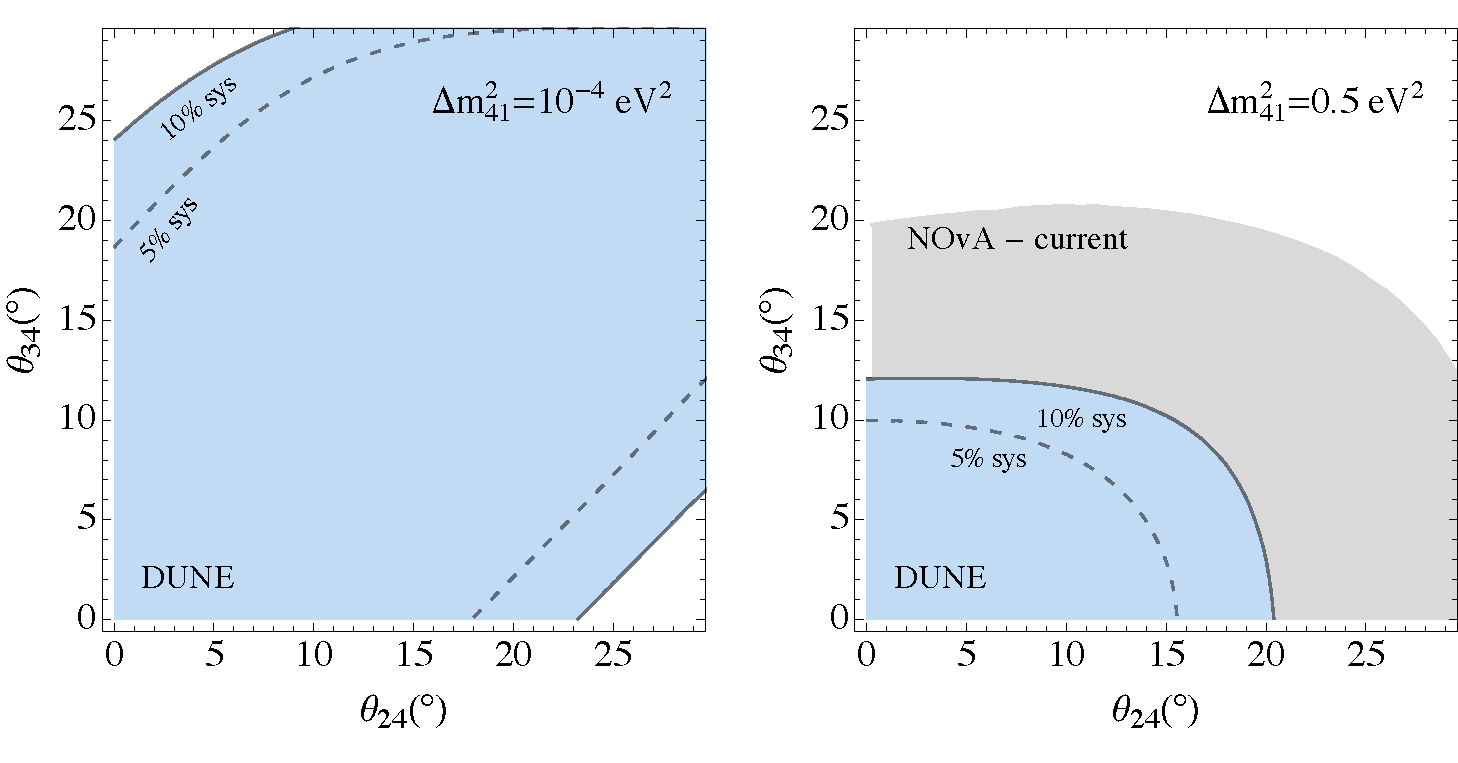
\includegraphics[scale=0.55]{plots/plot-th24-th34.pdf}
	\caption{Expected sensitivity projected in the $\theta_{24} - \theta_{34}$	plane, for an active-sterile mass-squared splitting $\Delta m^2_{41} = 10^{-4}$~eV$^2$ (left panel) and for $\Delta m^2_{41} = 0.5$~eV$^2$ (right panel). The shaded regions correspond to the expected confidence regions allowed at 90\% C.L. (2 d.o.f.), for a simulation assuming $\theta_{i4}=0$ as true input values. The lines labeled as ``10\% sys'' (``5\% sys'') have been obtained assuming 10\% (5\%) prior uncertainties for the signal (both shape and normalization) and 10\% for the background (normalization only).  Taken from Ref.~\cite{Coloma:2017ptb}.}
	\label{fig:sterile}
    \end{figure} 
        %
        \item Sterile neutrinos are another recurrent subject within the neutrino community. The mass of the extra neutrinos can span different energy scales from eV to TeV, and therefore have different phenomenological consequences. In particular, motivated by several anomalies, the hypothesis of an sterile neutrino at the eV scale is under investigation. This hypothesis has been tested in short and long baseline neutrino experiments without clear evidence, constraining the parameter space for the simplest 3+1 scheme. It is expected that a definitive test of this hypothesis would come from the results of future facilities like the short baseline neutrino program at FERMILAB and/or long-baseline facilities like DUNE. Efforts on this area are being done by the researchers from the Colombian community, for instance, looking for the possible constrains that could be obtained by the DUNE experiment to the additional mixing angles that appear in the case of a 3+1-neutrinos framework, through the observation of neutral current events at the far detector, as shown in Fig.~\ref{fig:sterile} (see Ref.~\cite{Coloma:2017ptb} and references there included).
        \item Several additional efforts are being pursued as part of the BSM physics working group at the DUNE collaboration. The Colombian community participate on the large extra-dimension searches at DUNE. For more details, we refer the reader to Ref.~\cite{Arguelles:2019xgp}.
    \end{itemize}
\end{enumerate}

\newpage
\bibliography{biblio} 
\end{document}
